\documentclass{article}

\usepackage[left=4cm, right=4cm]{geometry}
\usepackage{palatino}%Fuente
\usepackage{eulervm}%Fuente
\usepackage{graphicx}%Imágenes
\usepackage{float}%Imágenes
\usepackage{subcaption}%Imágenes
\usepackage{enumitem}%Listas
\usepackage{parskip}%Espacio entre párrafos
\usepackage{multicol}
\usepackage{amsthm,thmtools,xcolor}
\usepackage{amssymb}%Mate
\usepackage{amsmath}%Mate
\usepackage{tikz}%Mate (diagramas)
\usepackage{dutchcal}
\usepackage{tikz-cd}
\usepackage{xcolor}
\definecolor{blue-violet}{rgb}{0.54, 0.17, 0.89}
\usetikzlibrary{%
	matrix,%
	calc,%
	arrows,%
	shapes,
	decorations.markings,backgrounds,calc,intersections
}
\usepackage[bookmarks,bookmarksopen,bookmarksdepth=3]{hyperref}
\usepackage{cleveref}
\hypersetup{%colores
	colorlinks=true,
	urlcolor=blue,
	linkcolor=magenta,
	citecolor=blue,
	filecolor=blue,
	urlbordercolor=white,
	linkbordercolor=white,
	citebordercolor=white,
	filebordercolor=white
}

\makeatletter %Hide section number
\def\@seccntformat#1{%
	\expandafter\ifx\csname c@#1\endcsname\c@section\else
	\csname the#1\endcsname\quad
	\fi}
\makeatother
\usepackage{sectsty}
\sectionfont{\fontsize{13}{20}\selectfont}

\usepackage[style=authortitle,backend=bibtex]{biblatex}
\addbibresource{complex-geometry.bib}

\definecolor{blue-violet}{rgb}{0.54, 0.17, 0.89}
\definecolor{azure}{rgb}{0.0, 0.5, 1.0}
\definecolor{green(ncs)}{rgb}{0.0, 0.62, 0.42}
\definecolor{forestgreen}{rgb}{0.13, 0.55, 0.13}
\definecolor{limegreen}{rgb}{0.2, 0.8, 0.2}
\definecolor{palatinateblue}{rgb}{0.15, 0.23, 0.89}
\definecolor{trueblue}{rgb}{0.0, 0.45, 0.81}
\definecolor{goldenyellow}{rgb}{1.0, 0.87, 0.0}
\definecolor{fashionfuchsia}{rgb}{0.96, 0.0, 0.63}
\definecolor{brightcerulean}{rgb}{0.11, 0.67, 0.84}
\definecolor{jonquil}{rgb}{0.98, 0.85, 0.37}
\definecolor{lavendermagenta}{rgb}{0.93, 0.51, 0.93}
\definecolor{peru}{rgb}{0.8, 0.52, 0.25}
\definecolor{persimmon}{rgb}{0.93, 0.35, 0.0}
\definecolor{persianred}{rgb}{0.8, 0.2, 0.2}
\definecolor{persianblue}{rgb}{0.11, 0.22, 0.73}
\definecolor{persiangreen}{rgb}{0.0, 0.65, 0.58}
\definecolor{persianyellow}{rgb}{0.9, 0.89, 0.0}

\theoremstyle{definition}

\declaretheoremstyle[headfont=\color{trueblue}\normalfont\bfseries,]{colored1}
\declaretheoremstyle[headfont=\color{forestgreen}\normalfont\bfseries,]{colored2}
\declaretheoremstyle[headfont=\color{peru}\normalfont\bfseries,]{colored3}
\declaretheoremstyle[headfont=\color{persiangreen}\normalfont\bfseries,]{colored4}
\declaretheoremstyle[headfont=\color{brightcerulean}\normalfont\bfseries,]{colored5}
\declaretheoremstyle[headfont=\color{lavendermagenta}\normalfont\bfseries,]{colored6}
\declaretheoremstyle[headfont=\color{blue-violet}\normalfont\bfseries,]{colored7}
\declaretheoremstyle[headfont=\color{green(ncs)}\normalfont\bfseries,]{colored8}
\declaretheoremstyle[headfont=\color{peru}\normalfont\bfseries,]{colored9}
\declaretheoremstyle[headfont=\color{persiangreen}\normalfont\bfseries,]{colored10}

\declaretheorem[style=colored1,numberwithin=section,name=Theorem]{thm}
\declaretheorem[style=colored2,numberwithin=section,numberlike=thm,name=Proposition]{prop}
\declaretheorem[style=colored3,numberwithin=section,numberlike=thm,name=Lemma]{lemma}
\declaretheorem[style=colored4,numberwithin=section,numberlike=thm,name=Corollary]{coro}
\declaretheorem[style=colored5,numbered=no,name=Example]{example}
\declaretheorem[style=colored5,numbered=no,name=Examples]{examples}
\declaretheorem[style=colored6,numbered=no,name=Exercise]{exercise}
\declaretheorem[style=colored7,numberwithin=section,name=Remark]{remark}
\declaretheorem[style=colored7,numberwithin=section,name=Observation]{obs}
\declaretheorem[style=colored9,numbered=no,name=Claim]{claim}
\declaretheorem[style=colored8,numbered=no,name=Definition]{defn}
\declaretheorem[style=colored10,numbered=no,name=Question]{question}

\numberwithin{equation}{section}

\newcommand{\A}{\mathbb{A}}
\newcommand{\R}{\mathbb{R}}
\newcommand{\Z}{\mathbb{Z}}
\newcommand{\N}{\mathbb{N}}
\newcommand{\C}{\mathbb{C}}
\newcommand{\Q}{\mathbb{Q}}
\newcommand{\D}{\mathbb{D}}
\renewcommand{\P}{\mathbb{P}}

\newcommand{\Ac}{\mathcal{A}}
\newcommand{\Bc}{\mathcal{B}}
\newcommand{\Cc}{\mathcal{C}}
\newcommand{\Dc}{\mathcal{D}}
\newcommand{\Ec}{\mathcal{E}}
\newcommand{\Fc}{\mathcal{F}}
\newcommand{\Gc}{\mathcal{G}}
\newcommand{\Hc}{\mathcal{H}}
\newcommand{\Ic}{\mathcal{I}}
\newcommand{\Jc}{\mathcal{J}}
\newcommand{\Kc}{\mathcal{K}}
\newcommand{\Lc}{\mathcal{L}}
\newcommand{\Mc}{\mathcal{M}}
\newcommand{\Nc}{\mathcal{N}}
\newcommand{\Oc}{\mathcal{O}}
\newcommand{\Pc}{\mathcal{P}}
\newcommand{\Qc}{\mathcal{Q}}
\newcommand{\Rc}{\mathcal{R}}
\newcommand{\Sc}{\mathcal{S}}
\newcommand{\Tc}{\mathcal{T}}
\newcommand{\Uc}{\mathcal{U}}
\newcommand{\Vc}{\mathcal{V}}
\newcommand{\Wc}{\mathcal{W}}
\newcommand{\Xc}{\mathcal{X}}
\newcommand{\Yc}{\mathcal{Y}}
\newcommand{\Zc}{\mathcal{Z}}

\newcommand{\mf}{\mathfrak{m}}
\newcommand{\Cinf}{C^\infty}

\DeclareMathOperator{\img}{img}
\DeclareMathOperator{\Arg}{Arg}
\DeclareMathOperator{\id}{id}
\DeclareMathOperator{\Alt}{Alt}
\DeclareMathOperator{\Spec}{Spec}
\DeclareMathOperator{\sgn}{sgn}
\DeclareMathOperator{\supp}{supp}
\DeclareMathOperator{\Int}{Int}
\DeclareMathOperator{\Ob}{Ob}
\DeclareMathOperator{\Mor}{Mor}
\DeclareMathOperator{\Top}{Top}
\DeclareMathOperator{\CGWH}{CGWH}
\DeclareMathOperator{\Hom}{Hom}
\DeclareMathOperator{\Map}{Map}
\DeclareMathOperator{\Tot}{Tot}
\DeclareMathOperator{\Vect}{Vect}
\DeclareMathOperator{\VectBund}{VectBund}
\DeclareMathOperator{\Open}{Open}
\DeclareMathOperator{\Ring}{Ring}
\DeclareMathOperator{\Set}{Set}
\DeclareMathOperator{\Sets}{Sets}
\DeclareMathOperator{\Ab}{Ab}
\DeclareMathOperator{\op}{op}
\DeclareMathOperator{\Groups}{Groups}
\DeclareMathOperator{\eq}{eq}
\DeclareMathOperator{\Fun}{Fun}
\DeclareMathOperator{\Coh}{Coh}
\DeclareMathOperator{\coker}{coker}
\DeclareMathOperator{\an}{an}
\DeclareMathOperator{\alg}{alg}
\DeclareMathOperator{\Pic}{Pic}


\begin{document}
{\Huge complex geometry}
\tableofcontents
\section{abstract nonsense}

\begin{defn}\leavevmode
	\begin{itemize}
		\item A \textbf{\textit{pullback}} of the morphisms $f$ and $g$ consists of an object $P$ and two morphisms $p_1:P\to X$ and $p_2:P\to Y$ satisfying the following universal property:
		\[\begin{tikzcd}
			Q\arrow[rrd,bend left,"q_2"]\arrow[ddr,"q_1",swap,bend right]\arrow[dr,dashed,"\phi"]\\
			&P\arrow[r,"p_2"] \arrow[rd, phantom, "\lrcorner", very near start]\arrow[d,"p_1",swap]&Y\arrow[d,"g"]\\
			&X\arrow[r,"f",swap]&Z
		\end{tikzcd}\]
		\item A \textbf{\textit{pushout}} of the morphisms $f$ and $g$ consists of an object $P$ and two morphisms $i_1:P\to X$ and $i_2:P\to Y$ satisfying the following universal property:
		\[\begin{tikzcd}
			Z\arrow[r,"g"]\arrow[d,swap,"f"]&Y\arrow[d,"i_2"]\arrow[ddr,bend left,"j_2"]\\
			X\arrow[r,"i_1",swap]\arrow[drr,bend right,swap,"j_1"]&P\arrow[ul, phantom, "\ulcorner", very near start]\arrow[dr,dashed,"\phi"]\\
			&&Q
		\end{tikzcd}\]
		\item A \textbf{\textit{product}} of $X$ and $Y$ is an object $X\sqcup Y$ and a pair of morphisms $p_1:X\sqcap Y\to X$, $p_2:X\sqcap Y\to Y$ satisfying the following universal property:
		\[\begin{tikzcd}
			Q\arrow[rrd,bend left,"q_2"]\arrow[ddr,"q_1",swap,bend right]\arrow[dr,dashed,"\phi"]\\
			&X\sqcap Y\arrow[r,"p_2"]\arrow[d,"p_1",swap]&Y\\
			&X
		\end{tikzcd}\]
		\item A \textbf{\textit{coporoduct}} of $X$ and $Y$ is an object $X\sqcup Y$ and a pair of morphisms $i_1:X\to X\sqcup Y$, $i_2:Y\to X\sqcup Y$ satisfying the following universal property:
		\[\begin{tikzcd}
			&Y\arrow[d,"i_2"]\arrow[ddr,bend left,"j_2"]\\
			X\arrow[r,"i_1",swap]\arrow[drr,bend right,swap,"j_1"]&X\sqcup Y\arrow[dr,dashed,"\phi"]\\
			&&Q
		\end{tikzcd}\]
		\item A morphism $i$ has the \textbf{\textit{left lifting property with respect to a morphism $p$}} and $p$ has the \textbf{\textit{right lifting property with respect to $i$}} if for each morphisms $f$ and $g$, if the outer square in the following diagram commutes, there exists $\phi$ (I think not necessarily unique) completing the diagram:
		\[\begin{tikzcd}[row sep=large]
			A\arrow[r,"f"]\arrow[d,"i",swap]&X\arrow[d,"p"]\\
			B\arrow[r,"g",swap]\arrow[ur,dashed,"\phi"]&Y
		\end{tikzcd}\]
		\item The \textbf{\textit{kernel}} of a morphism is that part of its domain which is sent to zero. Formally, in a category with an initial object 0 and pullbacks, the \textbf{\textit{kernel $\ker f$}} of a morphism $f:A\to B$ is the pullback $\ker(f)\to A$ along $f$ of the unique morphism $0\to B$
		
		More explicitly, this characterizes the object $\ker(f)$ as \textit{the} object (unique up to isomorphism) that satisfies the following universal property:
		\begin{quote}
			for every object $C$ and every morphism $h:C\to A$ such that $f\circ h=0$ is the zero morphism, there is a unique morphism $\phi:C\to\ker(f)$ such that $h=p\circ\phi$.
		\end{quote}
		\[\begin{tikzcd}
			C\arrow[dr,dashed,"\phi"]\arrow[ddr,bend right,swap,"h"]\\
			&\ker(f)\arrow[d]\arrow[r]&0\arrow[d]\\
			&A\arrow[r,"f",swap]&B\arrow[ul, phantom, "\ulcorner", very near start]
		\end{tikzcd}\]
		\item In a category with a terminal object 1, the \textbf{\textit{cokernel}} of a morphism $f:A\to B$ is the pushout (arrows $h$ and $\phi$ apply if terminal object is zero)
		\[\coker(f):=1\sqcup_AB\qquad\qquad\begin{tikzcd}
			A\arrow[r,"f"]\arrow[d]\arrow[dr, phantom, "\lrcorner", very near start]&B\arrow[d]\arrow[rdd,bend left,"h"]\\
			1\arrow[r]&\coker(f)\arrow[dr,dashed,"\phi"]\\
			&&C
		\end{tikzcd}\]
		In the case when the terminal object is in fact zero object, one can, more explicitly, characterize the object $\coker(f)$ with the following universal property:
		\begin{quote}
			for every object $C$ and every morphism $h:B\to C$ such that $h\circ f=0$ is the zero morphism, there is a unique morphism $\phi:\coker(f)\to C$ such that $h=\phi\circ i$.
		\end{quote}
		
		\item A morphism $f:X\to Y$ is a \textbf{\textit{monomorphism}} if for every object $Z$ and every pair of morphisms $g_1,g_2:Z\to X$ then
		\[f\circ g_1=f\circ g_2\implies g_1=g_2.\]
		\[\begin{tikzcd}
			Z\arrow[r,shift={(0,.06)},"g_1"]\arrow[r,swap,shift={(0,-.06)},"g_2"]\arrow[rr,bend left,"f\circ g_1"]\arrow[rr,bend right,swap,"f\circ g_2"]&X\arrow[r,"f"]&Y
		\end{tikzcd}\]
		Equivalently, $f$ is a monomorphism if for every $Z$ the hom-functor $\Hom(Z,-)$ takes it to an injective function
		\[\begin{tikzcd}
			\Hom(Z,X)\arrow[r,hook,"f_*"]&\Hom(Z,Y).
		\end{tikzcd}\]
		Being a monomorphism in a category $\Cc$ means equivalently that it is an epimorphism in the opposite category $\Cc^{\op}$.
		
		\item A morphism $f:X\to Y$ is a \textbf{\textit{epimorphism}} if for every object $Z$ and every pair of morphisms $g_1,g_2:Y\to Z$ then
		\[g_1\circ f=g_2\circ f\implies g_1=g_2.\]
		\[\begin{tikzcd}
			X\arrow[r,"f"]\arrow[rr,bend right,swap,"g_2\circ f"]\arrow[rr,bend left,"g_1\circ f"]&Y\arrow[r,shift={(0,.06)},"g_1"]\arrow[r,swap,shift={(0,-.06)},"g_2"]&Z
		\end{tikzcd}\]
		Equivalently, $f$ is a epimorphism if for every $Z$ the hom-functor $\Hom(-,Z)$ takes it to an injective function
		\[\begin{tikzcd}
			\Hom(Y,Z)\arrow[r,hook,"f^*"]&\Hom(X,Z).
		\end{tikzcd}\]
		Being a monomorphism in a category $\Cc$ means equivalently that it is an monomorphism in the opposite category $\Cc^{\op}$.
	\end{itemize}
\end{defn}
\section{sheaf cohomology}
This section is (almost) literally \cite{huybrechts} appendix B.

In the following, $M$ will be a topological space. In most of the examples it is a differential or complex manifold.
\begin{defn}
	A \textbf{\textit{pre-sheaf $\Fc$}} of abelian groups (or vector spaces, rings, etc.) on $M$ consists of an abelian group (resp. vecot space, ring, etc.) $\Gamma(U,\Fc)=\Fc(U)$ for every open subset $U\subset M$ and a group homomorphism (resp. linear map, ring homomorphism, etc.) $r_{U,V}:\Fc(V)\to \Fc(U)$ for any two nested open subsets $U\subset V$ satisfying the following two conditions:
	\begin{enumerate}
		\item[$(i)$] $r_{U,U}=\id_{\Fc(U)}$.
		\item[$(ii)$] For open subsets $U\subset V\subset W$ one has $r_{U,V}\circ r_{V,W}=r_{U,V}$.
	\end{enumerate}
	Sometimes, one additionally requires $\Fc(\varnothing)=0$. In order to lighten the notation a bit, one may also write $s|_U$ instead of $r_{U,V}(s)$.
\end{defn}
\begin{example}
	The basic example is $\Fc=\Cc_M^0$, the pre-sheaf of continuous functions on $M$. More precisely, $\Cc_M^0(U)$ is the ring of all continuous maps $f:U\to\R$.
\end{example}
For $\Fc=\Cc_M^0$ one easily verifies the following additional conditions which do not hold for arbitrary pre-sheaves. We let $U=\bigcup U_i$ be the union of open subsets $U_i\subset M$. Then 
\begin{enumerate}
	\item[$(iii)$] If $f,g\in\Cc^0_M\left(\bigcup U_i\right)$ with $r_{U_i,U}(f)=r_{U_i,U}(g)$ for all $i$, then $f=g$.
	\item[$(iv)$] If functions $f_i\in\Cc_M^0(U_i)$ are given for all $i$ such that $r_{U_i\cap U_j,U_i}(f_i)=r_{U_i\cap U_j,U_j}(f_j)$ for any $j$, then there exists a continuous function $f\in\Cc^0_M(U)$ with $r_{U_i,U}(f)=f_i$ for all $i$.
\end{enumerate}
This leads to the definition of a sheaf.

\begin{defn}
	A pre-sheaf $\Fc$ is called a \textbf{\textit{sheaf}} if $(iii)$ and $(iv)$ are satisfied.
\end{defn}
\begin{examples}\leavevmode
	\begin{itemize}
		\item The constant pre-sheaf $\R$, for which $\Fc(U)=\R$ for all open subsets $\varnothing\neq U\subset M$ is not a sheaf as soon as $M$ contains a disconnected open subset. So, one works rather with the \textbf{\textit{constant sheaf(!) $\underline{\R}$}}, which, on an open set $U\subset M$ yields the set of all continuous functions $f:U\to\R$, where $\R$ is endowed with the discrete topology.
	
		Of course, one defines in the same manner constant sheaves associated to other vector spaces, groups, rings, etc.
		\item Another important example is the sheaf $\Ec$ of sections of a (topological) vector bundle $\pi:E\to M$. By definition, $\Ec(U)$ is the set of all (continuous) maps $s:U\to E$ with $\pi\circ s=\id_U$.
		
		In fact $\Ec$ is sheaf of $\Cc_M^0$-modules, that is, each $\Ec(U)$ is a $\Cc_M^0(U)$-module and the restriction maps are comparible with the module structures on the different open subsets.
		
		Since the vector bundle $E$ can be recovered from its sheaf of sections $\Ec$, one often uses the same notation $E$ for both.
	\end{itemize}
\end{examples}

\begin{defn}
	Let $\Fc$ and $\Gc$ be two (pre-)sheaves. A \textbf{\textit{(pre-)sheaf homomorphism}} $\varphi:\Fc\to\Gc$ is given by group homomorphisms (linear maps, ring homomorphisms, etc.) $\varphi_U:\Fc(U)\to\Gc(U)$ for any open subset $U\subset M$ satisfying $r_{U,V}^{\Gc}\circ \varphi_V=\varphi_U\circ r_{U,V}^{\Fc}$ for any $U\subset V$.
\end{defn}
Once a homomorphism $\varphi:\Fc\to \Gc$ of (pre-)sheaves of abelian groups is given, one constructs the associated pre-sheaves $\ker(\varphi)$, $\img(\varphi)$ and $\coker(\varphi)$ which are defined in the obvious way, that is, $\coker(\varphi)(U)=\coker(\varphi_U:\Fc(U)\to\Gc(U))$.

There is an important subtlety here. If $\varphi$ is a sheaf homomorphism then $\ker(\varphi)$ is a sheaf itself, but $\img(\varphi)$ and $\coker(\varphi)$, in general, are just pre-sheaves. In order to define the cokernel and the image of a sheaf homomorphism as honest sheaves, one needs to introduce the notion of a stalk.
\begin{defn}
	Let $\Fc$ be a (pre-)sheaf on $M$ and $x\in M$. Then the \textbf{\textit{stalk}} of $\Fc$ at $x$ is
	\[\Fc_x:=\{(U,s):x\in U\subset M,s\in\Fc(U)\}/\sim\]
	Here, for two open subsets $U_i$, $i=1,2$ and sections $s_i\in\Fc(U_i)$, $i=1,2$, one sets $(U_1,s_1)\sim(U_2,s_2)$ if there exists an open subset $x\in U\subset U_1\cap U_2$ such that $r_{U,U_1}(s_1)=r_{U,U_2}(s_2)$.
	
	Equivelently, one could introduce the stalk $\Fc_x$ as the direct limit $\Fc_x=\lim_{x\in U}\Fc(U)$.
\end{defn}
\begin{remark}
	One immediatly finds that any section $s\in\Fc(U)$ induces an element $s_x\in\Fc_x$ for any point $x\in U$. Furthermore, any (pre-)sheaf homomorphism $\varphi:\Fc\to\Gc$ induces homomorphisms $\Fc_x\to\Gc_x$ for any $x\in M$.
\end{remark}
\begin{defn}
	The \textbf{\textit{sheaf $\Fc^+$ associated to a pre-sheaf $\Fc$}} is the sheaf for which $\Fc^+(U)$ of an open subset $U\subset M$ is the set of all maps $s:U\to\bigcup_{x\in U}\Fc_x$ with $s(x)\in\Fc_x$ and such that for all $x\in U$ there exists an open subset $x\in V\subset U$ and a section $t\in\Fc(V)$ with $s(y)=t(y)$ for all $y\in V$. {\color{magenta}what?}
\end{defn}
\begin{remark}
	With this definition, $\Fc^+$ is a sheaf and the natural inclusion $\Fc\subset\Fc^+$ is an isomorphism if the pre-sheaf $\Fc$ was already a sheaf. For many constructions one needs to pass from a naturally defined pre-sheaf to its \textbf{\textit{sheafification}}. For example, the tensor product $\Fc\otimes_{\Rc}\Gc$ of two $\Rc$-modules $\Fc$ and $\Gc$ is defined as the sheafification of $U\mapsto\Fc(U)\otimes_{\Rc(U)}\Gc(U)$.
\end{remark}

\begin{defn}
	Let $\varphi:\Fc\to\Gc$ be a homomorphism of sheaves. Then the \textbf{\textit{image sheaf $\img(\varphi)$}} is the sheaf associated with the image pre-sheaf $U\mapsto\img(\varphi_U)$. Analogously, one defines the \textbf{\textit{cokernel sheaf $\coker(\varphi)$}}.
\end{defn}
\begin{defn}
	The sheaf homomorphism $\varphi$ is \textbf{\textit{injective}} if and only if $\ker(\varphi)$ is trivial. Similarly, one says that $\varphi$ is \textbf{\textit{surjective}} if its cokernel sheaf $\coker(\varphi)$ is trivial.
\end{defn}
	The essential difference between the two properties is that $\varphi$ is injective if and only if $\varphi_U$ is injective for any open set $U$. On the other hand, $\varphi$ might be surjective without $\varphi_U$ being surjective for all/any open subset. However, both properties can be detected by ther stalks. More precisely,
\begin{quote}
	$\varphi$ is injective or surjective if and only if $\varphi_x:\Fc_x\to\Gc_x$ is injective respectively surjective for any point $x\in M$.
\end{quote}
\begin{defn}
	A sequence $\Fc^\bullet$ of sheaf homomorphisms
	\[\begin{tikzcd}
		\cdots\arrow[r]&\Fc^i\arrow[r,"\varphi^i"]&\Fc^{i+1}\arrow[r,"\varphi^{i+1}"]&\Fc^{i+2}\arrow[r,"\varphi^{i+2}"]&\cdots
	\end{tikzcd}\]
	is a \textbf{\textit{complex}} if $\varphi^{i+1}\circ\varphi^i=0$ for all $i$. It is in an \textbf{\textit{exact complex}} if $\ker\varphi^{i+1}=\img\varphi^i$ for all $i$.
	
	An exact complex of the form \begin{tikzcd}
		0\arrow[r]&\Fc^0\arrow[r]&\Fc^1\arrow[r]&\Fc^2\arrow[r]&0
	\end{tikzcd} is called \textbf{\textit{short exact sequence}}.
\end{defn}
\begin{coro}
	A complex of the form
	\[\begin{tikzcd}
		0\arrow[r]&\Fc^0\arrow[r]&\Fc^1\arrow[r]&\Fc^2\arrow[r]&0
	\end{tikzcd}\]
	is exact if and only if the induced complex of stalks
	\[ \begin{tikzcd}
		0\arrow[r]&\Fc_x^0\arrow[r]&\Fc_x^1\arrow[r]&\Fc_x^2\arrow[r]&0
	\end{tikzcd}\]
	is exact for any $x\in M$.
\end{coro}
\begin{remark}
	Since surjectivity does not mean surjectivity for any open subset, a short exact sequence as above does not necessarily define short exact sequences
	\[ \begin{tikzcd}
		0\arrow[r]&\Fc^0(U)\arrow[r]&\Fc^1(U)\arrow[r]&\Fc^2(U)\arrow[r]&0
	\end{tikzcd}\]
	for any subset $U\subset M$ and in particular not for $M$. \textbf{This is where cohomology comes in.} It turns out that the failure of surjectivity of $\Fc^1(M)\to\Fc^2(M)$ is measured by the cohomology of $\Fc^0$.
\end{remark}

In order to introduce sheaf cohomology, one has to make a choice. There is the theoretically superior but rather abstract approach via derived categories or the more ad hoc one using acyclic resolutions. We outline the second one.

One first has to single out special sheaves with no cohomology in order to define cohomology for all other ones by resolving them.

\begin{defn}
	A \textbf{\textit{resolution}} of a sheaf $\Fc$ is a complex  \begin{tikzcd}
		0\arrow[r]&\Fc^0\arrow[r]&\Fc^1\arrow[r]&\Fc^2\arrow[r]&0
	\end{tikzcd} together with a homomorphism $\Fc\to\Fc^0$ such that
	\[\begin{tikzcd}
		0\arrow[r]&\Fc\arrow[r]&\Fc^0\arrow[r]&\Fc^1\arrow[r]&\Fc^2\arrow[r]&\cdots
	\end{tikzcd}\]
	is an exact complex of sheaves.
\end{defn}
One possible choice for sheaves without cohomology is provided by flasque sheaves.
\begin{defn}
	A sheaf $\Fc$ is called \textbf{\textit{flasque}} if for any open subset $U\subset M$ the restriction map $r_{U,M}:\Fc(M)\to\Fc(U)$ is surjective.
\end{defn}
Why flasque sheaves are the right ones is explained by the following
\begin{lemma}\label{lem:flasque}
	If
	\[\begin{tikzcd}
		0\arrow[r]&\Fc^0\arrow[r]&\Fc^1\arrow[r]&\Fc^2\arrow[r]&0
	\end{tikzcd}\]
	is a short exact sequence and $\Fc^0$ is flasque, then the induced sequence
	\[\begin{tikzcd}
		0\arrow[r]&\Fc^0(U)\arrow[r]&\Fc^1(U)\arrow[r]&\Fc^2(U)\arrow[r]&0
	\end{tikzcd}\]
	is exact for any open subset $U\subset M$.
\end{lemma}
Next, one has to ensure that any sheaf can be resolved by flasque sheaves. This will allow to define the cohomology of any sheaf.
\begin{prop}\label{prop:flasque-resolutions}
	Any sheaf $\Fc$ on $M$ admits a resolution
	\[\begin{tikzcd}
		0\arrow[r]&\Fc\arrow[r]&\Fc^0\arrow[r]&\Fc^1\arrow[r]&\Fc^2\arrow[r]&\cdots
	\end{tikzcd}\]
	such that all sheaves $\Fc^i$, $i=0,1,\ldots$ are flasque.
\end{prop}
\begin{defn}
	The \textbf{\textit{$i$-th cohomology group $H^i(M,\Fc)$}} of a sheaf $\Fc$ is the $i$-th cohomology of the complex
	\[\begin{tikzcd}
		\Fc^0(M)\arrow[r,"\varphi^0"]&\Fc^1(M)\arrow[r,"\varphi^1"]&\Fc^2(M)\arrow[r,"\varphi^2"]&\cdots
	\end{tikzcd}\]
	{\color{cyan}induced by a flasque resolution} $\Fc\to\Fc^\bullet$. Explicitly,
	\[H^i(M,\Fc)=\dfrac{\ker(\varphi^i_M:\Fc^i(M)\to\Fc^{i+1}(M))}{\img(\varphi^{i-1}_M:\Fc^{i-1}(M)\to\Fc^i(M))}\]
\end{defn}
Clearly, with this definition any flasque sheaf $\Fc$ has vanishing cohomology $H^i(M,\Fc)=0$ for $i>0$. (This is because of \cref{lem:flasque}: though it is stated as a \textit{short} exact sequence, it certainly implies exactness at every arrow in a long exact sequence of flasque sheaves.)

Moreover, for any sheaf $\Fc$ one has $\ker\varphi_M^0=H^0(M,\Fc)=\Gamma(M,\Fc)=\Fc(M)$. Indeed, in virtue of \cref{prop:flasque-resolutions}, \[\img(\Fc\to\Fc^0)=\ker(\Fc^0\to\Fc^1)\]
as sheaves, that is, as the sheafifications of the pre-sheaves
\[U\mapsto\img (\varphi_U:\Fc(U)\to\Fc^0(U))\quad \text{and}\quad U\mapsto\ker(\varphi^0_U:\Fc^0(U)\to\Fc^1(U))\]
calling the first arrow $\varphi$ for now. Taking $U=M$, we simply have that
\[\img\varphi_M=\ker\varphi^0_M\]
and $\varphi_M:\Fc(M)\to\Fc^0(M)$ injectively so that $\img\varphi_M\cong\Fc(M)$.

That this definition of cohomology is really independent of the chosen fiasque resolution is due to
\begin{prop}
	If $\Fc\to\Fc^\bullet$ and $\Fc\to\Gc^\bullet$ are two flasque resolutions of a sheaf $\Fc$ then both define naturally isomorphic cohomology groups.
\end{prop}

The most striking feature of cohomology is that it explains fully the non­ exactness of short exact sequences on the level of global sections.
\begin{prop}
	Let
	\[\begin{tikzcd}
		0\arrow[r]&\Fc^0\arrow[r]&\Fc^1\arrow[r]&\Fc^2\arrow[r]&0
	\end{tikzcd}\]
\end{prop}
	
\section{coherent sheaves}

\begin{defn}A sheaf of $A$-modules $\Fc$ over a sheaf of rings $A$ (on a topological space $X$) is called
	\begin{itemize}
		\item \textbf{\textit{locally finitely generated}} or \textbf{\textit{of finite type}} if there is a covering of $X$ by $U_i$, such that modules $F(U_i)$ are finitely generated over rings $A(U_i)$, i.e. over open subset $U_i$ there is a finite number $n_i$ and a surjective homomorphisms (over $U_i$) of $A$-modules: 
		\[A \otimes \C^{n_i}\twoheadrightarrow F\to 0,\] in principle for different $U_i$ they can be unrelated to each other.   For brevity I denote $A \otimes C^{n_i}$ by $A^n$.
		
		\item \textbf{\textit{locally finitely presented}} if there is a covering as above such that the respective modules are finitely presented over respective rings, that is  locally there is an exact sequence 
		\[A^m\to A^n\twoheadrightarrow F\to 0\]
		where $m$ and $n$ may depend on $i$, in other words locally $F$ is isomorphic to a cokernel of a homomorphism between free finitely generated $A$-modules.
		
		\item \textbf{\textit{coherent}} if it is locally finitely generated, and also for any finite $n$ and a local homomorphism $h : A^n \to F$ its kernel $\ker h$ is locally finitely generated sheaf of $A$-modules. Note that coherence obviously implies locally finitely presentedness,  consider $h_i : A^{n_i} \to F$ to be the surjective local (over $U_i$) homomorphisms that guarantee local finited generatedness of $F$, coherence implies their kernels are finitely generated by $m_i$ elements i.e. $A^{m_i} \twoheadrightarrow \ker h_i$, so take the composition $A^{m_i}\twoheadrightarrow \ker h_i \to A^{n_i}$ and notice it gives a local presentation of $F$, i.e. an exact sequence $A^{m_i} \to A^{n_i}\twoheadrightarrow F\to 0$.

		\item \textbf{\textit{locally noetherian}} if for any $U$ and any increasing sequence of sheaves of submodules $F_k$ of $F$, there is a covering of $U$ by $U_i$ such that on each $U_i$ the sequence $F_k$ stabilizes. 
	\end{itemize}
\end{defn}
\begin{defn}
	A sheaf of rings $A$ over a topological space $X$ (i.e.  a ringed space $(X,A)$ is called
	
	\begin{itemize}
		\item  \textbf{\textit{coherent}}, if it is coherent as a sheaf of $A$-modules (modules over itself).
		
		\item  \textbf{\textit{locally noetherian}} if it is locally noetherian as a sheaf of $A$-modules.
	\end{itemize}
\end{defn}
Notice that if a sheaf of rings (X,A) is locally noetherian, then  it is automatically coherent.
\begin{prop}
	If a sheaf of rings $A$ is coherent, then any l.f.g.l.f.p. (locally finitely generated and locally finitely presented) sheaf of $A$-modules is coherent.
\end{prop}
\begin{remark}
	Usually Hilbert basis theorem is proved in some form that if $A$ is Noetherian then polynomials $A[x]$ and formal power series $A[[x]]$ are Noetherian rings.
	
	In particular, $\C[x]$ and $\C[[x]]$ are Noetherian rings, as well as a ring of power series of non-zero radius of convergence (ring of stalks of functions holomorphic in 0).
\end{remark}
\begin{exercise}
	In contrast, ring of everywhere convergent power series, that is the ring of entire functions, is not Noetherian — simple exercise, use e.g. ideals generated by inverse $\Gamma$ function and its shifts by integers $1/\Gamma(s-n)$. Neither holomorphic functions over a disc or other Stein manifolds.
\end{exercise}
Nevertheless, 
\begin{thm}[Oka's coherence theorem]
	The ring of everywhere convergent power series, that is the ring of entire functions, is coherent.
\end{thm}
\begin{coro}
	Complex manifolds are coherent spaces.
\end{coro}
Coherence is a property strictly weaker than Noetherianness, and \textit{in complex analytic geometry there are no local noetherian spaces, but nevertheless all spaces are local coherent and this is sufficient for doing geometry}.

\begin{defn}
	There is a notion of \textbf{\textit{global finite generatedness}}, that says there is a surjection $\Oc_X^n \twoheadrightarrow F \to 0$ (over whole of $X$).
\end{defn}
\begin{remark}
	The condition of being finitely generated implies that
	\[\Oc_{X,n}\twoheadrightarrow F_x\to 0\qquad\forall x\in X\]
	simply because surjectivity (more generally, exactness) of maps of sheaves is true iff it is true for every stalk.
	
	In other direction this is probably not true (for ringed spaces in general), without extra condition (such as F being of finite type, so making cyclic loops, or noetherianness of $X$, but this would be too strong).
\end{remark}
\begin{thm}[Cartan's theorem A]
	Analytic / algebraic coherent sheaves over Stein / affine varieties are globally finitely generated.
\end{thm}

Over more general bases this is obviously wrong, e.g. look for anti-ample line bundles over projective spaces, e.g. $\Oc_{\P^1}(-1)$ that we considered earlier. But the result (Theorem A, and also Theorem B) is very useful for the 'gears' of the theory.

In contrast, locally finitely generated means there is a covering, that restrictions are f.g. over these subsets. Or equivalently, for any point there is a neighbourhood that restriction is f.g. in this neighbourhood.

\begin{defn}
	Let $Z\subset X$ be a closed subset of a scheme $X$, $z\in Z$, $U$ an open set containing $z$ and $f_1,\ldots,f_n\in\Oc_{X,z}$ a finite collections of locally holomorphic functions such that $Z\cap U$ is the zeroes of $f_1,\ldots,f_n$. The \textbf{\textit{ideal sheaf}} of $Z$ is given by
	\[\Ic(U)=\{f\in\Oc(U):\forall z\in Z\cap U, f\in(f_1,\ldots,f_n)\}\]
\end{defn}
\paragraph{4 coherence theorems}
\begin{thm}
	Oka's
\end{thm}
\begin{thm}
	$Z\subset X$ a $\C$ analytic subvariety, then $\Ic_Z\in \Coh(X)$.
\end{thm}
\begin{thm}
	Grauert-Reinmart.
\end{thm}
\begin{thm}[Grauert's direct image theorem]
	If $f:X\to Y$ if proper and $\Fc\in\Coh(X)$, then $f_*\Fc\in\Coh(X)$ and $\forall i \;R^i f_*\Fc\in\Coh Y$. (+ hom to relate )
\end{thm}
\clearpage

\section{abelian categories}
\begin{defn}
	A category is \textbf{\textit{pre-additive}} if $\Hom_\Cc(M,N):=\Cc(M,N)$ has a structure of abelian groups, that is, $\Cc(M,N)$ is an abelian group and composition $\Cc(M,N)\times\Cc(N,L)\to\Cc(M,K)$ is bilinear. So
	\[\begin{tikzcd}[column sep=huge]
		&\Ab\arrow[d]\\
	\Cc^{\op}\times\Cc\arrow[r,"\Hom(-\text{,}-)",swap]\arrow[ur,dashed]&\Set
\	\end{tikzcd}\]
\end{defn}
\begin{defn}
	$(X,\eta)$ is called a \textbf{\textit{group object}} in a category $\Cc$ if it is addionally equipped with a lift
	\[\begin{tikzcd}
		&\Groups\arrow[d]\\		\Cc^{\op}\arrow[r,"h_x",swap]\arrow[ur,"\eta",dashed]&\Sets
	\end{tikzcd}\]
	where $h_x=\Hom(-,X)$.
\end{defn}
\begin{exercise}
	What is a group object in a category of groups?
\end{exercise}
\begin{defn}
	Usually, an \textbf{\textit{abelian category}} is a pre-additive category that has
	\begin{itemize}
		\item Limits
		\begin{enumerate}
			\item Products.
			\item Equalizers, equivalently, kernels. Since $\eq(f,g)=\ker(f-g)$ and $\ker(f)=\eq(f,0)$.
		\end{enumerate}
		\item Colimits
		\begin{enumerate}
			\item Coproducts.
			\item Coequalizers (cokernels).
		\end{enumerate}
	\end{itemize}
\end{defn}
\begin{lemma}[Yoneda]
	$h:\Cc\to\Fun(\Cc^{\op},\Sets)$ naturally.
\end{lemma}
\begin{examples}
	content...
\end{examples}
\begin{defn}
	$\img(f)=\ker(\coker(f))$
\end{defn}
\begin{defn}
	Additive functor.
\end{defn}
\begin{defn}
	Short exact sequence, complexes.
\end{defn}
\begin{remark}
	For any complex $K$ in $\Ac$ and additive functor $F:\Ac\to\Bc$, $F(K)$ is a complex.
\end{remark}
\begin{defn}
	\begin{itemize}
		\item $F$ is \textbf{\textit{biexact}} if it preserves exact sequences.
		\item $F:\Ac\to\Bc$ is \textbf{\textit{left-exact}} if 
		\begin{equation}\label{eq:exact}
			\begin{tikzcd}
			0\arrow[r]&A_1\arrow[r]&A_2\arrow[r]&A_3\arrow[r]&0
		\end{tikzcd}
		\end{equation}
		goes to
		\[\begin{tikzcd}
			0\arrow[r]&FA_1\arrow[r]&FA_2\arrow[r]&FA_3\arrow[r,phantom]& \leavevmode
		\end{tikzcd}\]
		where exacteness is allowed to fail in the last term.
		\item $F:\Ac\to\Bc$ is \textbf{\textit{right-exact}} if \cref{eq:exact} is mapped to
		\[\begin{tikzcd}
			\leavevmode\arrow[r,phantom]&FA_1\arrow[r]&FA_2\arrow[r]&FA_3\arrow[r]& 0
		\end{tikzcd}\]
		where exacteness is allowed to fail in the first term.
	\end{itemize}
\end{defn}

\section{derived functors}
Consider the functor of global sections $\Gamma:\Ab(X)\to\Ab$. It is additive and left-exacts. Its derived functors are called cohomology.

To compute $H^k(X,\Fc)$ we can use a resolution of $\Fc$ by \textbf{\textit{acyclic objects}} (with no higher cohomology).

\begin{claim}
	For any short exact sequence of sheaves
	\[\begin{tikzcd}
		0\arrow[r]&\Fc\arrow[r]&\Gc\arrow[r]&\Hc\arrow[r]&0
	\end{tikzcd}\]
	induces a long exact sequence on homology.
\end{claim}

\begin{example}
	Consider the exact sequence
	\[\begin{tikzcd}[row sep=tiny]
		0\arrow[r]&\Z\arrow[r]&\Oc_X^{\an}\arrow[r]&\Oc_X^{*\an}\arrow[r]&0\\
		&1\arrow[r,maps to]&f\arrow[r,maps to]&\exp(2\pi if)
	\end{tikzcd}\]
	where $\Oc_X^{*\an}$ is the sheaf of invertible analytic functions, which is not an $\Oc_X$-module and therefore not coherent (while $\Oc_X^{\an}$ is).

	Let us find
	\begin{itemize}
		\item $H^k(X,\Z)$, Betti (singular) cohomology.
		\item $H^k(X,\Oc_X^{\an})$.
		\item $H^k(X,\Oc^{*\an}_X)$.
	\end{itemize}
	\begin{claim}
		$H^1(X,\Oc_X^{*\an})=\Pic(X^{\an})$, the abelian group of holomorphic line bundles.
		
		Moreover, the statement holds for algebraic functions and algebraic line bundles, that is, $H^1(X,\Oc_X^{*\alg})=\Pic(X^{\alg})$.
	\end{claim}
	\begin{defn}
		Let $\Fc$ be a sheaf of abelian groups. The \textbf{\v Cech cohomology cochain} is
		\[\check{C}(X,\Fc;\{U_i\}_{i\in I})=\bigoplus_{\substack{J\subset I\\|J|=k+1}}\Fc(U_J)\cdot\Z\]
		with differential
		\begin{align*}
			d:\check{C}^k&\to\check{C}^{k+1}\\
			\Fc(U_J)&\mapsto \Fc(U_{J})
		\end{align*}
		and several other properties
	\end{defn}
	Anyway, the following map in the long exact sequence concerning this example
	\[\begin{tikzcd}[row sep=tiny]
		H^1(X,\Oc^{\an}_X)\arrow[r]&H^1(X,\Oc^{\an}_X)=\Pic(X)\arrow[r,magenta]&H^2(X,\Z)\arrow[r]&H^2(X,\Oc^{\an}_X)\\
		&\Lc\arrow[r,maps to]&c_1(\Lc)
	\end{tikzcd}\]
	is called the \textbf{\textit{first Chern class}}.
	
	Moral: if $H^k(X,\Oc_X^{\an})=0$ for $k=1$ and $k=2$ then $c_1$ gives an isomorphism of holomorphic line bundles to topological line bundles.
\end{example}

\begin{example}
	If $X$ is Stein, for example $X^{\an}$ for $X$ affine, then Cartan Theorem B says that $H^k(X,\Fc)=0$ for all $k>0$ , $\Fc\in\Coh\Fc$. So Oka+Cartan imply $H^k(X,\Oc_X^{\an})=0$ for all $k>0$.
	
	So, \textit{Cartan B $\implies$ $c_1$ is isomorfism if $X^{\an}$ is Stein}.
\end{example}
\begin{example}[subexample]
	If $X$ is an affine curve then $\Pic^{\an}X^{\an}=0$ but $\Pic^{\alg}X$ is huge (if $g(x)>0$) (anti GAGA).
\end{example}
\begin{example}
	If $X$ is Fano, ($\omega^*_X=\det\Gamma_X$), Kodaira embedding theorem, Kodaira Vanishing theorem.
\end{example}

\begin{example}
	Consider the exact sequence
	\[\begin{tikzcd}[row sep=tiny]
		0\arrow[r]&\Z\arrow[r]&\Oc_X^{\Cinf}\arrow[r]&\Oc_X^{*\Cinf}\arrow[r]&0\\
		&1\arrow[r,maps to]&f\arrow[r,maps to]&\exp(2\pi if)
	\end{tikzcd}\]
	where $\Oc_X^{*\Cinf}$ is the sheaf of invertible analytic functions, which is not an $\Oc_X$-module and therefore not coherent ({\color{magenta}while $\Oc_X^{\Cinf}$ is?}).
	
	Let us find
	\begin{itemize}
		\item $H^k(X,\Z)$, Betti (singular) cohomology.
		\item $H^k(X,\Oc_X^{\Cinf})$.
		\item $H^k(X,\Oc^{*\Cinf}_X)$.
	\end{itemize}
	Like before, the map in the middle within the long exact sequence
	\[\begin{tikzcd}[row sep=tiny]
		H^1(X,\Oc^{\Cinf}_X)\arrow[r]&H^1(X,\Oc^{*\Cinf}_X)\arrow[r]&H^2(X,\Z)\arrow[r]&H^2(X,\Oc^{\Cinf}_X)
	\end{tikzcd}\]
	is also called the \textbf{\textit{first Chern class}} (and you could also call $H^1(X,\Oc^{*\Cinf}_X)$ the \textbf{\textit{smooth Picard module}}).
	
	Important thing is that $\Oc_X^{\Cinf}$ is \textbf{\textit{fine}}. Also any sheaf of $\Oc_X^{\Cinf}$-modules is fine. So the groups in the far left and far right in the sequence above are zero, so the first chern class is an isomorphism.
	
	\begin{coro}
		If $\Fc$ is a cheaf of $\Cinf_X$-modules, then it is acyclic, that is $H^k(X,\Fc)=0\;\forall k>0$.
	\end{coro}
\end{example}
\begin{remark}
	So we have that Cartan B implies that $\Pic X^{\an}=0$, but $\Pic^{\alg}\cong X$.
\end{remark}

\section{line bundles and divisors}
There's a correspondence between line bundles and divisors.
\begin{defn}\leavevmode
	\begin{itemize}
		\item Morally, \textbf{\textit{divisors}} are formal linear combinations of irreducible Weil divisors (irreducible algebraic subvarieties of codimension 1), $\sum_{\text{finite}}a_iD_i$ with $a_i\in\Z$.
		\item \textbf{\textit{Cartier divisors}} are the ones that are \textit{locally} given as divisors of \textit{rational function ones}. That means that there is (or maybe, \textit{it is}) a covering $\Uc=\{U_i\}$ and on each $U_i$ one is given by $\varphi_i=p_i/q_i$, where
		\item a \textbf{\textit{meromorphic function on $U$}} is given by $U=\bigcup V_i$ with $V_i$ connected, so on $V_i$ pick two homolorphic functions $p_i,q_i$ such that $q_i\not\equiv0$, then the meromorphic function is $\varphi_i=p_i/q_i$. So on $U_{ij}$ we have that $\varphi_i=\varphi_j$, that is $p_iq_i=p_jq_j$.
	
		\textit{So I don't ask that the two functions coincide in the intersection, but rather that the quotient is holomorphic in the intersection.}
	\end{itemize}
\end{defn}
\begin{remark}\leavevmode
	\begin{itemize}
		\item Cartier divisors $\subset$ Weil divisors.
		\item So there's the analogy between regular functions which are quotients of polynomials and meromorphic functions which are quotients of holomorphic functions.
	\end{itemize}
\end{remark}
\begin{example}\leavevmode
	\begin{itemize}
		\item $X$=$\frac{\Spec\C[x,y,z]}{(xy-z^2)}$. Consider $D=L=\{x=z=0\}$. From \href{https://en.wikipedia.org/wiki/Divisor_(algebraic_geometry)}{Wikipedia}:
		
		\begin{quote}
			Let $X$ be the quadric cone of dimension 2, defined by the equation $xy = z^2$ in affine 3-space over a field. Then the line $D$ in $X$ defined by $x = z = 0$ is not principal on $X$ near the origin. Note that $D$ can be defined as a set by one equation on $X$, namely $x = 0$; but the function $x$ on $X$ vanishes to order 2 along D, and so we only find that $2D$ is Cartier (as defined below) on $X$. In fact, the divisor class group $\operatorname{Cl}(X)$ is isomorphic to the cyclic group $\Z/2$, generated by the class of $D$.[Hartshorne example II.6.5.2]
		\end{quote}
		\begin{figure}[H]
			\centering
			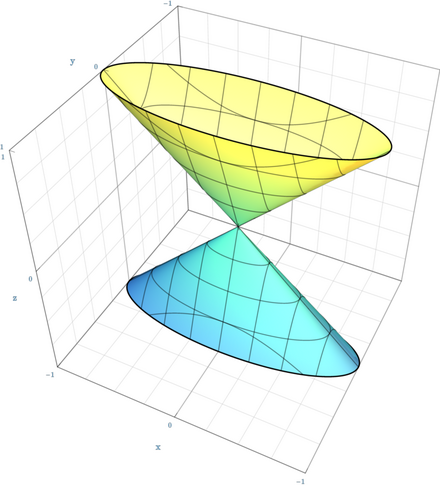
\includegraphics[width=0.7\linewidth]{divisor}
			\caption{$xy=z^2$}
			\label{fig:divisor}
		\end{figure}
		
		\item $X$=$\frac{\Spec\C[x,y,z,w]}{(xy-zw)}$. So $D=L=\{x=z=0\}$.
	\end{itemize}
\end{example}
\begin{defn}
	$D$ is \textbf{\textit{Q-Cartier}} if there exists $N$ such that $ND$ is Cartier.
\end{defn}
\begin{prop}
	No multiple of $D_1$ is Cartier.
\end{prop}
\addcontentsline{toc}{section}{References}
\printbibliography
\end{document}